%%%%%%%%%%%%%%%%%%%%%%%%%%%%%%%%%%%%%%%%%
% Formal Text-Rich Title Page 
% LaTeX Template
% Version 1.0 (27/12/12)
%
% This template has been downloaded from:
% http://www.LaTeXTemplates.com
%
% Original author:
% Peter Wilson (herries.press@earthlink.net)
%
% License:
% CC BY-NC-SA 3.0 (http://creativecommons.org/licenses/by-nc-sa/3.0/)
% 
% Instructions for using this template:
% This title page compiles as is. If you wish to include this title page in 
% another document, you will need to copy everything before 
% \begin{document} into the preamble of your document. The title page is
% then included using \titleGP within your document.
%
%%%%%%%%%%%%%%%%%%%%%%%%%%%%%%%%%%%%%%%%%

%----------------------------------------------------------------------------------------
%	PACKAGES AND OTHER DOCUMENT CONFIGURATIONS
%----------------------------------------------------------------------------------------

\documentclass{book}
\usepackage{graphicx}
\usepackage{dirtytalk}
\usepackage{fancyhdr}
\usepackage{wrapfig}
\usepackage[normalem]{ulem}
\usepackage[utf8]{inputenc}
\usepackage[T1]{fontenc}
\usepackage[table]{xcolor}

\pagestyle{fancy}
\fancyhead[LE,RO]{}
\fancyhead[RE,LO]{\rightmark}
\fancyfoot[CE,CO]{\leftmark}
\fancyfoot[LE,RO]{\thepage}
\fancyfoot[RE,LO]{ZENG FAN PU, 2016}
\renewcommand{\headrulewidth}{2pt}
\renewcommand{\footrulewidth}{1pt}




\newcommand*{\plogo}{\fbox{$\mathcal{VTX}$}} % Generic publisher logo

%----------------------------------------------------------------------------------------
%	TITLE PAGE
%----------------------------------------------------------------------------------------

\newcommand*{\titleGP}{\begingroup % Create the command for including the title page in the document
\centering % Center all text
%\vspace*{\baselineskip} % White space at the top of the page

\rule{\textwidth}{1.6pt}\vspace*{-\baselineskip}\vspace*{2pt} % Thick horizontal line
\rule{\textwidth}{0.4pt}\\[\baselineskip] % Thin horizontal line

 {\Huge ARS RHETORICA}\\ {\Large COMPILED FOR \\[0.3\baselineskip] THE NEW SAT (ESSAY)}\\[0.2\baselineskip] % Title

\rule{\textwidth}{0.4pt}\vspace*{-\baselineskip}\vspace{3.2pt} % Thin horizontal line
\rule{\textwidth}{1.6pt}\\[\baselineskip] % Thick horizontal line

\scshape % Small caps-0
A number of fascinating and life-changing explanations and examples \\ % Tagline(s) or further description
presented  in a clear and useable way \\[\baselineskip] % Tagline(s) or further description

\vspace*{1\baselineskip} % Whitespace between location/year and editors

Written by \\[\baselineskip]
{\Large ZENG FAN PU\par} % Editor list
{\itshape Hwa Chong Institution \\ Singapore\par} % Editor affiliation

\vspace*{\baselineskip} % Whitespace between location/year and editors
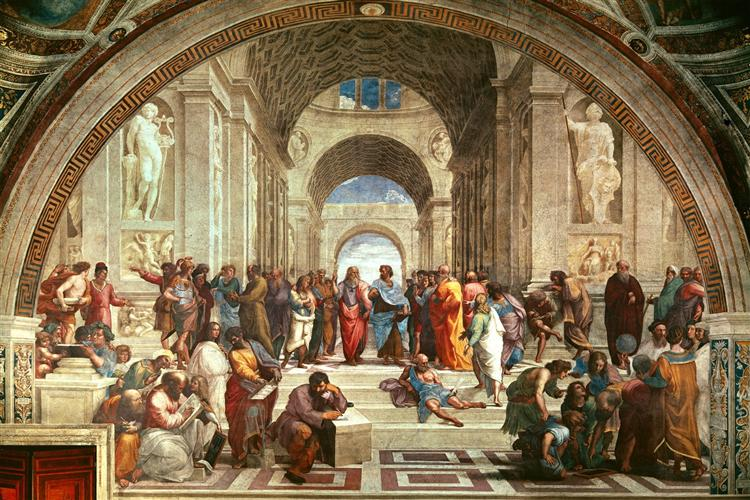
\includegraphics[scale=0.6]{SchoolOfAthens}

\vfill % Whitespace between editor names and publisher logo

\plogo \\[0.3\baselineskip] % Publisher logo
{\scshape 2016} \\[0.3\baselineskip] % Year published
{\large VORTEX PUBLISHINGS}\par % Publisher

\endgroup}

%----------------------------------------------------------------------------------------
%	BLANK DOCUMENT
%----------------------------------------------------------------------------------------

\begin{document} 
\thispagestyle{empty}
%\pagestyle{empty} % Removes page numbers

\titleGP % This command includes the title page
\pagenumbering{arabic}
\setcounter{tocdepth}{4}

\tableofcontents
\chapter{Rhetoric}
\section{Overview}

\begin{itemize}
	\item Set your \textbf{goals} and the argument's \textbf{tense}
	\item Think of whether you want to emphasize \textbf{character}, \textbf{logic}, or \textbf{emotion}
	\item Make sure the \textbf{time} and the \textbf{medium} are ripe for persuasion
\end{itemize}

\textbf{Cicero's speech outline:}
\begin{enumerate}
	\item Introduction
	\item Narration
	\item Division
	\item Proof
	\item Refutation
	\item Conclusion
\end{enumerate}

\section{Goals}
\subsection{Personal Goal}
What you want from your audience
\subsection{Audience Goals}
\begin{itemize}
	\item Mood: This is the easiest thing to change
	\item Mind: A step up in difficulty from changing the mood
	\item Willingness to act: Hardest of all, because it requires an emotional commitment and identification with the action 
\end{itemize}

\subsection{Issue control} 
Mastering argument's chief topics
\begin{itemize}
	\item Blame (Forensic): Covers the past. Its chief topics are \emph{guilt} and \emph{innocence}
	\item Values (Demonstrative): Get argued in the present tense. Chief topics are \emph{praise} and \emph{blame}.
	\item Choice (Deliberative): Deals with the future. Its chief topic is the \emph{advantageous} - what's best for the audience.
\end{itemize}

\section{Ethos}
This is argument by character - using your reputation or someone else's as the basis for argument. When you give a speech, play up your character - or what you want the audience to think it is. Its three chief aspects are virtue (areté), practical wisdom (phronesis), and disinterest (eunoia). Ethos is widely considered by scholars to be the most important appeal.\\

\subsection{Decorum}
Your ability to fit in with the audience's expectation of a trustworthy leader.
\begin{itemize}
	\item Code Grooming: Using language unique to the audience
	\item Identity Strategy: It makes the audience think of your choices as expressions of the group, helping them identify with the action. Anyone who chooses otherwise risks feeling separated from the pack. 
	\item Irony: Saying one thing to outsiders with a meaning revealed only to your group.
	\item Use of Diction: Intentionally simple and succint or elaborate and jargon-laden to appeal to the knowledge base of the audience.
\end{itemize}

\textbf{\emph{By mastering the art of fitting in, [author] is able to present himself as the ideal leader of the [cause] with his proposals sounding like the collective consensus of the audience, cueing anyone who identifies with the [cause] to take up his suggestions or risk feeling alienated. 
}}
\subsection{Virtue, or Cause}
The appearance of living up to your audience's values, areté.
\begin{itemize}
	\item Bragging: The straightforward, and least effective, way to enhance your virtue
	\item Witness Bragging: An endorsement by a third party, the more disinterested the better
	\item Tactical Flaw: A defect or mistake, intentionally revealed, that shows your rhetorical virtue
	\item Switching Sides: Appearing to have supported the powers that be all along
	\item Throwing the support behind the inevitable: Enthusiastically endorse the opponent's view to show off your virtue. Only use if you're bound to lose anyway.
	\item Logic-free Values: Focusing on the individual values-words and commonplaces to bring a group together and get it to identify with you.
	\item Identity: Get people to describe themselves. Usually the first thing they mention reveals their best sense of who they are. And most people will do just about anything to live up to that identity.
	\item The Halo: Sum up the issue in a few words. Suss out the values of your audience. Now, find a representative or piece of the issue that can symbolize those values.
\end{itemize}

\emph{\textbf{When [the audience|readers] come to see that [author] share their set of values and beliefs, he becomes more trustworthy in their eyes, seeing him as the standard bearer who is championing their interests.}}

\subsection{Practical Wisdom, or Craft}
Phronesis, a type of wisdom relevant to practical things, requiring an ability to discern how or why to act virtuously and encourage practical virtue, excellence of character, in others.

\begin{itemize}
	\item Showing off experience
	\item Bending the rules
	\item Appearing to take the middle course
\end{itemize}

\textbf{\emph{By demonstrating that he is well versed in the field through [techniques used], [author's name] is able to build up his credibility and increase the weight of his words, making [the audience|readers] more amenable to his [suggestions|opinions].}}

\subsection{Disinterest, or Caring}
Eunoia - an apparent willingness to sacrifice your own interests for the greater good, ``disinterested goodwill''.], which combines selflessness and likeability.
\begin{itemize}
	\item Reluctant Conclusion: Appearing to have reached your conclusion only because of its overwhelming rightness, despite your own desires for the contrary.
	\item Personal Sacrifice: Claiming that the choice will help your audience more than it will help you.
	\item Dubitatio: Seeming doubtful of your own rhetorical skill
	\item Considering both sides: Anticipate the audience's objections and produce them even before the audience can. This makes listeners more malleable. They begin to assume that you'll take care of all their qualms, and lapse into a state of persuadability.
\end{itemize}

\textbf{\emph{[Author] successfully proves that he understands the pain and concerns of his audience and makes them believe that [he has nothing personal at stake/he is nobly self-sacrificing by arguing for a stance that is apparently contrary to his own interests]. Hence his only motivation for [his stance] is due to its overwhelming rightness, inducing the audience to [appreciate his goodwill and go along with his suggestions/be afflicted with a tinge of guilt if they do not support [his cause] in view of his sacrifices].}}


\subsection{Liar detector}
Techniques for judging a person's credibility. (Rarely applicable in SAT)
\begin{itemize}
	\item Needs Test: Do the persuader's needs match your needs?
	\item Comparable Experience: Has the persuader actually done what he's talking about?
	\item Dodged Question: Ask who benefits from the choice. If you don't get a straight answer, don't trust that person's disinterest.
	\item `That depends' Filter: Instead of a one-size-fits-all choice, the persuader offers a solution tailored to you.
	\item `Sussing' Ability: The persuade cuts to the chase of an issue.
	\item Extremes: How does the persuader describe the opposing argument? How close is his middle-of-the-road to yours?
	\item Extremist Detector: An extremist will describe a moderate choice as extreme.
	\item Virtue Yardstick: Does the persuader find the sweet spot between the extremes of your values?
	\item Code Inoculation: Be aware of the terms that define the groups you belong to, anmd watch out when a persuader uses them.
\end{itemize}

\subsection{Screw-up Recovery}
Enhancing your ethos through your own mistakes. (Rarely applicable in SAT)
\begin{itemize}
	\item Set your goals right after you screw up
	\item Be first with the news
	\item Switch immediately to the future
	\item Avoid belittling the victim
	\item Don't apologize. Instead, express your feelings about not living up to your standards.
\end{itemize}

\section{Pathos}
Argument by emotion is the seductive part of persuasion. Pathos can cause a mood change, make an audience more receptive to your logic, and give them an emotional commitment to your goal. The seat of the emotions, the limbic system, tends to overpower the more rational parts of the brain, making it an even more powerful tool of persuasion than logos. Emotion comes from experience and expectation - what your audience believes has happened, or will take place in the future. The more vividly one gives the audience the sensations of an experience, the greater the emotion one can arouse.

\subsection{Sympathy}
Registering concern for your audience's emotions.
\begin{itemize}
	\item Oversympathizing: Exaggerated sympathy can make your audience feel ashamed of an emotion you want to change.
\end{itemize}

\subsection{Belief}
This is the key to emotion.
\begin{itemize}
	\item Experience: Refer to the audience's own experience, or plant one in their heads; this is the past tense of belief.
	\item Storytelling: A way to give the audience a virtual experience. See \emph{enargeia}.
	\item Expectation: Make an audience expect something good or bad, and the appropriate emotion will follow.
\end{itemize}

\subsection{Volume Control}
Underplaying an emotion, or gradually increasing it so that the audience can feel it along with you
\begin{itemize}
	\item Simple speech: Don't use fancy language when you get emotional.
	
\emph{\textbf{By [speaking|writing] simply, less is more, and the audience gains the impression that his words are spontaneous rather than premeditated as elaborate [speech|writing] is usually [rehearsed|planned] in advance, thereby increasing the authenticity of his emotions.
}}\end{itemize}

\subsection{Enargeia}
When a speaker describes an event so vividly, in such detail, that it seems as though the event is happening right in front of the audience.

\textbf{\emph{By describing the event so vividly and in such detail, [author] is able to evoke an experience and its concomitant sensations in the minds of [the audience|readers], which naturally arouses emotions of [emotions that the author wishes to create].}}

\subsection{Unannounced Emotion}
Avoid tipping off your audience in advance of a mood. They'll resist it.

\subsection{Passive Voice}
If you want to direct an audience's anger away from someone, imply that the action happened on its own: ``The chair got broken,'' not ``Pablo broke the chair.''

\emph{\textbf{His use of the passive voice seems to imply that the action happened on its own, helping to calm the passions and encourage passivity [so that readers will not take action (which supports his cause)].}}

\subsection{Backfire}
You can calm an individual's emotion in advance by overplaying it yourself. This works especially well when you screw up and want to prevent the wrath of an authority.

\subsection{Persuasive Emotions}
\begin{itemize}
	\item Anger: One of the most effective ways to rouse an aud ience to action. But it's a short-lived emotion.
	\item Belittlement Charge: Show your opponent disrespecting your audience's desires. A belittled audience is an angry one.
	
\emph{\textbf{[Author] shows that [opponent] has [disrespected/ridiculed the audience's desires|neglected the audience's problems|failed to take the audience's interests seriously], making them feel belittled. A belittled audience is an angry one, which empowers them to readily reject [opponent's claims].}}

	\item Patriotism: Attaches a choice or action to the audience's sense of group identity. Usually triggered by something negative - you get patriotic when your group is under threat.
	
\textbf{\emph{	He rouses feelings of patroitism in his [audience|readers] by showing [a rival group's success(negative)|the impending loss of prestige(negative)|something to be proud of(positive)] and promotes [his choice] as an avenue to express that patroitism.}}	
	
	\item Emulation: Emotional response to a role model. The greater your ethos, the more the audience will imitate you.
	\item Humor: A good calming device that can enhance your ethos.
		\begin{itemize}
			\item Urbane Humor: Plays off a word or part of speech.
			\item Wit: Situational Humor.
			\item Facetious Humor: Joke telling, a relatively ineffective form of persuasion.
			\item Banter: Snappy answers - works best in defense.
		\end{itemize}
		
\emph{\textbf{His witty remark temporarily disarms readers, breaking down their inherent antagonism for new ideas and therefore making them more amenable to his cause.}}
\end{itemize}

\subsection{Identity}
Discern people's best sense of who they are (their identity), and get them to identify with your choice. Most people will do just about anything to live up to that identity. The idea is to plant an image in your audience's head, associated with their values, that influences their outlook on an issue.

\begin{itemize}
	\item Define the issue in the plainest possible terms.
	\item Find the values.
	\item Symbolize the values. The idea is to take the issue as you've defined it, then extract a little piece of the issue to form a powerful symbol (trope).
\end{itemize}

\emph{\textbf{An identity is people's best sense of who they are. [Author] appeals to the [audience's|reader's] identity by framing his proposal in a way that is congruent with it. [Elaborate how]. He shows that his suggestions are not only congruent to that identity, but are of paramount importance to be taken up by [the audience] if they are to stay true to it. Most people will do just about anything to live up to their identity, causing the audience to eagerly adopt his recommendations.}}

\subsection{Empowerment}
When the audience is angry or belittled, make them feel powerful. Give them a sense of self-control. This can be achieved by utilising deliberative rhetoric.

\subsection{Figures of Speech}
\begin{itemize}
	\item Cliché Twisting: Using overworked language to your advantage.
		\begin{itemize}
			\item Literal Interpretation: Reducing a cliché to absurdity by seeming to take it at face value.
			\item Surprise Ending: Starting a cliché as it's normally said, but ending it differently.
			\item Reworking: Switching words around in a cliché
		\end{itemize}
	\item Word Swap: Changing normal usage and grammar for effect.
		\begin{itemize}
			\item Chiasmus: Creates a crisscross sentence.
		\end{itemize}
	\item Weighing both sides: Comparing or contrasting opinions in order to define the issue.
		\begin{itemize}
			\item Either/Or Figure (Dialysis): Weighs each side equally.
			
			\textit{``You're either for us, or against us.''}
			\item Contrasting Figure (Antithesis): Emphasizes the difference between the two ideas.
			
			\textit{``The success of our economy has always depended not just on the size of our gross domestic product, but on the reach of our prosperity...'' (Barack Obama)}
			\item Meaning-change Figure (Antistasis): Repeats a word in a way that uses or defines it differently. 
			
			\textit{``He that composes himself is wiser than he that composes a book." (Benjamin Franklin)}
		\end{itemize}
	\item Editing Out Loud: Interrupting yourself or your opponent to correct something.
		\begin{itemize}
			\item Self-correction Figure (Metanoia): Lets you amplify an argument while seeming to be fair and accurate.
			\item Redefiner (Correctio): Repeats the opponent's language and corrects it.
		\end{itemize}
	\item Volume Control: Amplifying or calming speech through figures.
		\begin{itemize}
			\item Ironic understatement. 
			
			\textit{``I lived at West Egg, the — well, the less fashionable of the two, though this is a most superficial tag to express the bizarre and not a little sinister contrast between them.'' (The Great Gatsby by F. Scott Fitzgerald)}
			\item Climax: Uses overlapping words in successive phrases in a rhetorical crescendo.
			
			\textbf{\emph{The author cites successive examples of [positive/negative consequences] as a result of [positive/negative situation], such as [evidence]. This entices readers to get into the rhythm of the cascade of [positive/negative events], anticipating and mentally filling in the next piece. Unbeknownst to the reader, he has led himself onto a slippery slope fallacy by continuously extrapolating the current trend, believing the [problem|situation] to be much [worse|better] than it actually will be.}}
			
		\end{itemize}
	\item Word Invention: Figures help you create new words or meanings from old words
		\begin{itemize}
			\item Verbing (Anthimeria): Turns a noun into a verb or vice versa.
			\item ``Like'' Figure (Parelcon): Strips a word of meaning and uses it as a pause or for emphasis. \emph{(``Like,'' ``You know,'')}
		\end{itemize}
\end{itemize}

\subsection{Simple Language}
Keeping to simple language and avoiding jargon helps to make your speech easy to comprehend, allowing audiences to follow closely without much thought. This strips them of the need to cogitate. They are then less likely to engage higher mental faculties such as skepticism, making them more docile and receptive to your ideas.

\section{Logos}
Argument by logic. People like to think that all argument should be nothing but logic; however, Aristotle said that when it comes to persuasion, rational speech needs emotion and character as well.

\subsection{Deduction}
Applying a general principle to a particular matter.

\emph{\textbf{[Author] employs sound deductive reasoning to prove [his cause]. He presents indubitable premises - [premise 1, 2, ...n]. Using the rule of modus ponens, one can immediately deduce that [conclusion] must be true.}}

\begin{itemize}
	\item Enthymeme: A logic sandwich that contains deduction. ``We should [choice], becuase [commonplace].'' Aristotle took formal logic's syllogism, stripped it down, and based it on a commonplace instead of a universal truth.
	\item Proof Spotter: A proof consists of examples or a premise. A premise usually begins with ``because,'' or implies it.
	\item Commonplace: Any cliche, belief, or value that can serve as your audience's boiled-down public opinion. It's the starting point of your argument.
		\begin{itemize}
			\item Babbling: An audience's repetition of a word or idea; it often reveals a commonplace.
			\item Rejection: Another good commonplace spotter. An audience will often use a commonplace when it rejects your argument.
			\item Commonplace Label: Applying a commonplace to an idea, a proposal, or a piece of legislation as part of a definition strategy.
		\end{itemize}
\end{itemize}

\subsection{Induction}
Argument by example. It starts with the specific and moves to the general. 

\emph{\textbf{[Author] utilises inductive reasoning to prove [his cause]. He raises [an example|a plethora of examples] of [the causes and consequences of (an) analagous case(s)], and one can easily generalise these occurences and safely assume based on [overwhelming evidence|the parallelism in context] that the same will also be true for [current situation].  
}}\begin{itemize}
	\item Fact, Comparison, Story: The three kinds of examples to use in inductive logic.
\end{itemize}

\subsection{Concession}
Using your opponent's own argument to your advantage.

\subsection{Framing}
Shaping the bounds of an argument. 

\begin{itemize}
	\item Framing Strategy
		\begin{enumerate}
			\item Find the audience's commonplaces.
			\item Define the issue broadly, appealing to the values of the widest audience.
			\item Deal with the specific problem or choice, using the future tense.
		\end{enumerate}
	\item Definition Strategy: Controlling the language used in an argument. Don't just accept your opponent's definition. Come up with your own instead. That way you sound as though you agree with your opponent's argument even while you cut the legs out from under it. 
	\item Term Change: Inserting your own language in place of your opponent's.
	\item Redefinition: Accepting your opponent's terms while changing their connotation.
	\item Definition Jujitsu: Using your opponent's language to attack him.
	\item Definition Judo: Using terms that contrast with your opponent's, creating a context that makes him look bad.
\end{itemize}

Framing in defense:
\begin{enumerate}
	\item If facts work in your favor, use them. If they don't or you don't know them,
	\item Redefine the terms instead. If that won't work, accept your opponent's facts and terms but
	\item Argue that your opponent's argument is less important than it seems. And if even that isn't to your advantage,
	\item Claim the discussion is irrelevant.
\end{enumerate}

\emph{\textbf{By virtue of his choice of words, [author] is able to frame the [issue] in a [positive|negative] light due to the subconscious connotations that such terms carry. [Examples]. He turns the issue from [negative|positive issue] to a [positive|negative issue]. Any fair-minded individual will see that the only reasonable choice to make is to [intended outcome by author].}}

\subsection{Logical Fallacies}

\begin{itemize}
	\item Bad Proof: The argument's commonplace or principle is unacceptable, or the examples are bad.
	\begin{itemize}
			\item False Comparison: Two things are similar, so they must be the same.
			\item Fallacy of Association: A is a member of group B. A is a member of group C. Therefore, group B is C. For example, natural ingredients are good for you, so anything called ``natural'' is healthful.
			\item Appeal to Popularity (Argumentum ad populum): Concludes that a proposition is true because many or most people believe it: ``If many believe so, it is so.''
			\item Hasty Generalization: Uses too few examples and interprets them too broadly
			\item Misinterpreting the Evidence: Takes the exception and claims it proves the rule.
			\item Unit Fallacy: Confusing the part for the whole
			\item Argument from Ignorance (Ad Ignorantium): Claims that if something has not been proven, it must be false.	
	\end{itemize}

	\item Bad Conclusion: We're given too many choices, or not enough, or the conclusion is irrelevant to the argument.
		\begin{itemize}
			\item Many Questions: Squashes two or more issues into a single one. Committed when someone asks a question that presupposes something that has not been proven or accepted by all the people involved.
			\item False Dilemma: Offers the audience two choices when more actually exist.
			\item Fallacy of Antecedent: If P, then Q. Therefore, not P, then not Q.
			\item Red Herring: Introduces an irrelevant issue to distract or confuse the audience. Eg. \emph{``There is a lot of commotion regarding saving the environment. We cannot make this world an Eden. What will happen if it does become Eden? Adam and Eve got bored there!''}
			\item Straw Man: Sets up a different issue that's easier to argue. Eg. \emph{``Obama's going to take all our guns!''}
		\end{itemize}
	\item Disconnect Between Proof and Conclusion: The proof stands up all right, but it fails to lead to the conclusion.
		\begin{itemize}
			\item Tautology: A logical redundancy; the proof and the conclusion are the same thing
			\item Reductio ad Absurdum: Takes the opponent's choice and reduces it to an absurdity
			\item Slippery Slope: Predicts a series of dire events stemming from one choice.
			\item Post Hoc Ergo Propter Hoc: Assumes that if one thing follows another, the first thing caused the second one.
		\end{itemize}
\end{itemize}

\emph{\textbf{[Author] astutely exposes logical fallacies in the arguments of his [opponent(s)|detractor(s)], who claim that [detractor's fallacious claim]. He shows that [flaw in opponent's reasoning]. This rebuttal not only rocks the foundations of his opponent's argument, but also invites the rest of his arguments to scrutiny and doubt, with grave repercussions on his opponent's logos and ethos.}}

\subsection{Rhetorical Fouls}
Mistakes or intentional offenses that stop an argument dead or make it fail to reach a consensus.
\begin{itemize}
	\item Switching Tenses Away From The Future: It's fine to use the past or present, but deliberative argument depends on eventually discussing the future.
	\item Inflexible Insistence On The Rules: Using the voice of God, sticking to your guns, refusing to hear the other side
	\item Humiliation: An argument that sets out only to debase someone, not to make a choice
	\item Innuendo: A form of irony used to debase someone. It often plants an idea in the audience's head by denying it.
	\item Threatening (Argumentum ad Baculum): It denies the audience a choice.
	\item Nasty Language or Signs
	\item Utter Stupidity
\end{itemize}

\section{Kairos}
The Romans called it occasio, the art of seizing the occasion. Kairos depends on timing and the medium.

\subsection{Persuadable Moment}
When the audience is ripest for your argument
\begin{itemize}
	\item Moment Spotter: Uncertain moods and beliefs - when minds are already beginning to change - signal a persuadable moment.
	\item Perfect Audience: Receptive, attentive, and well disposed toward you
	\item Audience Change: If the current audience isn't ready for persuasion, seek another one. This is what market research is all about.
\end{itemize}

\subsection{Senses}
The five senses are key to the proper medium.
\begin{itemize}
	\item Sight: Mostly pathos and ethos
	\item Sound: The most logical sense
	\item Smell, Taste and Touch: Almost purely emotional
\end{itemize}

\section{Speechmaking}
\subsection{Invention}
The crafting part of a speech. Its tools are the tools of logos.

\subsection{Arrangement}
The organization of a speech. Ethos first, then logos, then pathos.
\begin{itemize}
	\item Introduction (Exordium): The ethos part, which wins you the interest and the good will of the audience. 
	\item Narration, or Statement of Facts: Tell the history of the matter or list your facts and figures. If you have time, do both. This part should be brief, clear, and plausible. Don't repeat yourself. State the facts in chronological order, but don't begin at the beginning of time - just the part that is relevant to the immediate argument. Don't startle the audience with ``believe it or not'' facts - this part should be predictable. What they hear should sound usual, expected, and natural.
	\item Division: List the points where you and your opponent agree and where you disagree. This is where you can get into definitions as well. It's a biologial issue. It's an ethical issue. It's a rights issue. It's a practical issue (what benefits our society the most?). It's a fairness issue. Division can actually help your ethos, if you use the reluctant conclusion.
	\item Proof: Here is where you get into your actual argument, setting out your argument packet (``We should do this because of that'') and your examples.
	\item Refutation: Destroy your opponent's (anticipated) arguments here.
	\item Conclusion: Restate your best points and, if you want, get a little emotional.
\end{itemize}

\subsection{Style}
Choice of words that make a speech attractive to the listener. The five virtues of style:
\begin{itemize}
	\item Proper Language: Use words that suit the occasion and your audience
	\item Clarity: Would the least informed reader understand it?
	\item Vividness (Enargeia): The ability to create a rhetorical reality before the audience's very eyes. Involves all five senses.
	\item Decorum: The art of fitting in. Behave the way your audience expects you to.
	\item Ornament: Rhythm of your voice and the cleverness of your words. Does it sound good when you read it aloud?
\end{itemize}
	
\subsection{Memory}
The ability to speak without notes.

\subsection{Delivery}
The action of giving a speech.
\begin{itemize}
	\item Voice: Should be loud enough for the room
	\item Gesture: The eyes are key, even in a large room, because they lead your other facial muscles. Use few hand gestures in a formal speech.
\end{itemize}

\chapter{Writing}
\section{Synonyms}
Commonly used terms and their synonyms.

\subsection{Author's Action}
\subsubsection{Putting forth an argument}
Put forward (a plan or suggestion) for consideration by others: \textbf{put forward, suggest, advance, offer, present, recommend, advocate, propound, proffer, posit}

Analyse and develop (an idea or principle) in detail: \textbf{describe, give an explanation of, make clear/plain/intelligible, spell out, elucidate, expound, explicate, delineate, clarify, throw light on, clear up, simplify, demonstrate, show, illustrate, unravel}

\subsubsection{Alluding}
Suggest or call attention to indirectly; hint at: \textbf{allude, hint at, imply, mention, touch on, refer to, suggest, mention in passing, make an allusion to}

\subsubsection{Conveying}
Mention indirectly or briefly: \textbf{indicate, state, declare, make (it) known, announce, communicate, mention, say, reveal, divulge, disclose, register, record, admit}

Convey (a thought or feeling) in words or by gestures and conduct: \textbf{express, communicate, convey, indicate, show, demonstrate, reveal, intimate, manifest, exhibit, evidence, put across/over, get across/over, articulate, voice, state, assert, proclaim, profess, say, tell, speak, mouth, point out; denote, illustrate, symbolize, signify, embody, evince, asseverate}

\subsubsection{Using a technique}
Make practical and effective use of: \textbf{utilize, employ, deploy, make use of, apply, practise, put to use, use, take advantage of, exploit, milk, tap}

\subsubsection{Attempting to perform an action}
Make an effort to achieve or complete (something difficult):
\textbf{try, strive, aim, venture, endeavour, seek, set out, make an effort, make every effort, spare no effort, undertake, embark on}

\subsection{Intended Effect}
\subsubsection{Building rhetorical virtue}
Become or make greater in size, amount, or degree. \emph{Add to}: \textbf{augment, supplement, top up, build up, enlarge, expand, extend, raise, elevate, inflate,
magnify, intensify, strengthen, amplify, heighten, escalate,
improve, make better, boost, ameliorate, enhance, enrich, upgrade, reinforce}
\emph{Grow}: \textbf{increase, enlarge, expand, rise, climb, escalate, improve, intensify, strengthen, heighten, extend, build up, accrue, accumulate}. 

Make or become better: \textbf{improve, better, upgrade, refine, enhance, boost, raise}

\subsubsection{Strengthening argument}
Make or become stronger: \textbf{strengthen, fortify, bolster, give strength to, give a boost to, boost, reinforce, toughen, cement, add to, fuel, renew, vitalize, give new energy to}

\subsection{Immediately}
At once; instantly: \textbf{immediately, without hesitation, directly, instantly, promptly, straight away, at once, right away, forthwith, in a flash, tout de suite}

\section{Extracts}
\subsection{Introduction}
[Author's name] [propounds|advocates] that [cause] [because|as it will|due to] [negative/positive consequences]. [He/she] augments the persuasiveness of her arguments by actively incorporating various rhetorical elements of ethos, logos and pathos in her [essay|speech], winning the hearts and minds of [his/her] audience to [support/take up his/her [cause|beliefs] | reject/disapprove of [opposing cause|beliefs]].

\subsection{Body}
\subsubsection{Ethos}
[Author] attempts to [establishe his credibility|win the respect of|build rapport with] his readers in a multitude of ways. 

[...] 

\noindent Through his character appeal, [author] is able to appear likeable and trustworthy, turning [the audience|readers] into a receptive one who [is|are] willing to trust his judgement.

\subsubsection{Logos}
[Author's] cunning usage of logos also plays a major role in augmenting the persuasiveness of his [essay|speech]. 

[...]

\noindent [Author's] impervious logic, coupled with his ability to [techniques used], provides for a very convincing case that [the audience|readers] will find difficult to repudiate.

\subsubsection{Pathos}
Finally, [author] expolits the persuasiveness of the pathetic appeal in order to sway his [audience|readers] into agreeing with him. 

[...]

\noindent His usage of pathos is ultimately the key to rousing the audience into going above and beyond mere agreement to a state of impassioned commitment, so as to further his cause of [cause].

\subsection{Conclusion}
All things considered, [author's name] has managed to pull off a rhetorically impressive piece with his adroit usage of the trinity of ethos, logos and pathos. He sets off by establishing his [credibility|expertise|goodwill|trustworthiness|likeability through [summary of techniques]. He then builds up an impregnable fortress of reasoning by [summary of techniques], skillfully refuting and shattering [reader's|the audience's] confidence in the validity of [his opponent's arguments] while demonstrating the soundness of his own. [Author's name] delivers the final blow when he plays his trump card, the emotional appeal, by [summary of techniques], speaking them to their hearts and spurring them to [agree with his claims|dismiss his detractor's claims|take action]. The cohesive interplay of these rhetorical techniques makes for not just delightful [reading|listening], but also for one to be hard pressed to [disagree with the author's claim|agree with the claims of his detractors].

\section{Linking Phrases}
\begin{tabular}{ | l | l | l | l |}
    \hline
    Listing & Giving Examples & Generalising \\ \hline
 First, second, third  & For example & In general\\
 First, furthermore, finally & For instance & Generally\\ 
 To begin, to conclude & As folllows & On the whole\\
 Next & That is & As a rule \\
 & In this case & For the most part \\
 & Namely & In most cases\\
 & In other words & Usually \\
 \hline
 Reinforcement & Result/Consequence & Similarity \\
 \hline
 Also & So & Equally \\
 Furthermore & As a result/consequence & Likewise \\
 Moreover & Accordingly & Similarly \\
 What is more & Consequently & Correspondingly \\
 In addition & Because of this/that & In the same way \\
 Besides & Thus \\
 Above all & Hence \\
 As well (as) & For this/that reason \\
 In the same way & So that \\
 Not only...but also & In that case \\
 & Under these circumstances \\
\hline
Highlighting & Reformulation & Expressing an alternative \\
\hline
In particular & In other words & Alternatively \\
Particularly & Rather & Rather \\
Especially & To put it more simply & On the other hand \\
Mainly & & The alternative is \\
& & Another possibility would be \\ 
\hline
Transition to a new point & Deduction & Contrast \\
\hline
Now & Then & Instead \\
As far as \emph{x} is concerned & In other words & Conversely \\
With regard/reference to & In that case & On the contrary \\
As for ... & Otherwise & In contrast \\
It follows that & This implies that... & In comparison \\
Turning to & If so/not \\
\hline
Summary & Stating the obvious & Concession \\
\hline
In conclusion & Obviously & However \\
To conclude & Clearly & Even though \\
In brief & Naturally & However much \\
To summarise & Of course & Nevertheless \\
Overall & As can be expected & Still \\
Therefore & Surely & Yet \\
& After all \\
\hline
\end{tabular}
    
\end{document}